%%%%%%%%%%%%%%%%%%%%%%%%%%%%%%%%%%%%%%%%%%%%%%%%%%%%%%%%%%%%%
%% HEADER
%%%%%%%%%%%%%%%%%%%%%%%%%%%%%%%%%%%%%%%%%%%%%%%%%%%%%%%%%%%%%
\documentclass[a4paper,11pt, openright]{book}

% Alternative Options:
% Base Font Size: 10pt / 11pt / 12pt


%% Language %%%%%%%%%%%%%%%%%%%%%%%%%%%%%%%%%%%%%%%%%%%%%%%%%
\usepackage[USenglish]{babel} %francais, polish, spanish, ...
\usepackage[T1]{fontenc}
\usepackage[ansinew]{inputenc}

\usepackage{lmodern} %Type1-font for non-english texts and characters

%%%%%%%%%%% margin %%%%%%%%%%%%%%%%%%%%%%%%%%%%%%%%%%%%%%%%%%
\usepackage[a4paper] {geometry}
\geometry{hmargin={3cm,2cm}}
%\geometry{hmargin=2.5cm,top=3cm,bottom=2.3cm}


%% Packages for Graphics & Figures %%%%%%%%%%%%%%%%%%%%%%%%%%
\usepackage{graphicx} %%For loading graphic files
\usepackage{caption}
\usepackage{subcaption} %%Subfigures inside a figure
\usepackage{pdflscape}
%\usepackage{pst-all} %%PSTricks - not useable with pdfLaTeX

%%%% SPACING %%%%
\renewcommand{\baselinestretch}{1}  %%%%%%% space between lines %%%%%
%\headsep = 10.mm
%\setlength{\parskip}{2.0ex plus0.5ex minus0.5ex}
												
%%%% COMMANDS %%%%
\renewcommand\title{Study and Analysis of Networks Flows}
\newcommand\name{\textsc{Denis Genon \& Victor Velghe}}
\newcommand\options{Artificial Intelligence}
\newcommand\supervisor{ \textsc{Yves Deville}}
\newcommand\readerone{ \textsc{Fran\çois Aubry}}
\newcommand\readertwo{ \textsc{Jean-Charles Delvenne}}
\newcommand\years{2015-2016}

%% Math Packages %%%%%%%%%%%%%%%%%%%%%%%%%%%%%%%%%%%%%%%%%%%%
\usepackage{amsmath}
\usepackage{amsthm}
\usepackage{amsfonts}
%\usepackage{algorithm}
%\usepackage[noend]{algpseudocode}
\usepackage[boxed]{algorithm2e}

%% Code Writing %%%%%%%%%%%%%%%%%%%%%%%%%%%%%%%%%%%%%%%%%%%%%
\usepackage{listings}
% "define" Scala
\lstdefinelanguage{scala}{
  morekeywords={abstract,case,catch,class,def,%
    do,else,extends,false,final,finally,%
    for,if,implicit,import,match,mixin,%
    new,null,object,override,package,%
    private,protected,requires,return,sealed,%
    super,this,throw,trait,true,try,%
    type,val,var,while,with,yield},
  otherkeywords={=>,<-,<\%,<:,>:,\#,@},
  sensitive=true,
  morecomment=[l]{//},
  morecomment=[n]{/*}{*/},
  morestring=[b]",
  morestring=[b]',
  morestring=[b]"""
}

\lstset{frame=tb,language=scala,aboveskip=3mm,belowskip=3mm,showstringspaces=false,columns=flexible,basicstyle={\small\ttfamily}}
\renewcommand{\lstlistingname}{Code}
%% Line Spacing %%%%%%%%%%%%%%%%%%%%%%%%%%%%%%%%%%%%%%%%%%%%%
\usepackage{setspace}
%\singlespacing        %% 1-spacing (default)
%\onehalfspacing       %% 1,5-spacing
%\doublespacing        %% 2-spacing


%% Other Packages %%%%%%%%%%%%%%%%%%%%%%%%%%%%%%%%%%%%%%%%%%%
\usepackage{url} %%for url in the bibliography
%\usepackage{bold-extra}

%%%%%%%%%%%%%%%%%%%%%%%%%%%%%%%%%%%%%%%%%%%%%%%%%%%%%%%%%%%%%
%% DOCUMENT
%%%%%%%%%%%%%%%%%%%%%%%%%%%%%%%%%%%%%%%%%%%%%%%%%%%%%%%%%%%%%
\begin{document}

\pagestyle{empty} %No headings for the first pages.


%% Title Page %%%%%%%%%%%%%%%%%%%%%%%%%%%%%%%%%%%%%%%%%%%%%%%
\newgeometry{hmargin=2.5cm,top=3cm,bottom=2.3cm}
%!TEX root = ../main.tex
%%%% COVER %%%%
\definecolor{UCLblue}{cmyk}{1.00,0.68,0.00,0.54}
\definecolor{EPLblue}{cmyk}{0.70,0.30,0.00,0.00}
\renewcommand\title{Study and Analysis of Network Flows}	% Titre du TFE
\newcommand\subtitle{Augmenting Path and Preflow-push algorithms}
\newcommand\nameone{Denis \textsc{Genon}}	% Nom de l'étudiant
\newcommand\nametwo{Victor \textsc{Velghe}}	% Nom du 2nd étudiant éventuel
\newcommand\speciality{Sciences Informatiques}		% Spécialité (mentioner l'une des options suivantes):
										% ingénieur civil biomédical
										% ingénieur civil en chimie et science des matériaux
										% ingénieur civil des constructions
										% sciences informatiques
										% ingénieur civil en informatique
										% ingénieur civil électricien
										% ingénieur civil électromécanicien
										% ingénieur civil en mathématiques appliquées
										% ingénieur civil mécanicien
										% ingénieur civil physicien
\newcommand\options{Artificial Intelligence}	% À mentioner si demandé par la commission de programme
\newcommand\supervisor{Yves \textsc{Deville}}	% Nom du promoteur
%%\newcommand\cosupervisor{Prénom \textsc{Nom}}	% Nom du co-promoteur éventuel
\newcommand\readerone{Fran\c cois \textsc{Aubry}}		% Nom du 1er lecteur
\newcommand\readertwo{Jean-Charles \textsc{Delvenne}}		% Nom du 2nd lecteur
%%\newcommand\readerthree{Prénom \textsc{Nom}}	% Nom du 3e lecteur éventuel
\newcommand\years{2015-2016}	% Année académique

% Création de la page de titre
\makeatletter
\renewcommand{\maketitle}
	{\begin{titlepage}
	\newgeometry{top=1.25cm,bottom=1.25cm,left=1.25cm,right=1.25cm}
	\begin{center}
		
\includegraphics[scale=1]{images/EPL_TFEbanner.jpg}
	\end{center}
	\vspace*{9pt}
	\begin{flushright}
	    \color{UCLblue} \fontfamily{phv} \selectfont
	    {\huge \title} \\
	    \vspace*{12pt}
	    {\Large \subtitle} \\
	    \vspace*{12pt}
		\large Dissertation presented by \\
		\textbf{\nameone}
		\textbf{, \nametwo}
		\\
		\vspace*{12pt} 
		for obtaining the Master's degree in \\
		\textbf{\speciality} \\
%		\textit{Option(s): \options}	% Uncomment if necessary
		\vspace*{12pt}
		Supervisor\\
		\textbf{\supervisor} 
%		\textbf{, \cosupervisor}		% Uncomment if necessary
		\\
		\vspace*{12pt}
		Readers \\
		\textbf{\readerone, \readertwo}
%		\textbf{, \readerthree}	% Uncomment if necessary
		\\
		\vspace*{12pt}
		Academic year \years \\
	\end{flushright}
	\vspace*{9pt}
	\color{EPLblue}{\rule{18.5cm}{8.25cm}}
  \end{titlepage}}
\makeatother


\maketitle					% To create front cover page
\thispagestyle{empty}		% To suppress header and footer on the back of the cover page


%%%% END COVER %%%%

\restoregeometry
\cleardoublepage
\section*{Abstract}
%!TEX root = ../main.tex
Ant Colony Optimization is a metaheuristic which mimics ants behavior to solve optimization problems. Ant Colony Optimization has proven to be very effective in various fields of applications. One inconvenient with ACO is the complex mapping of a problem into something that can be used by this metaheuristic. Also, adapting an ACO application from one problem to another is difficult and requires a lot of programming efforts. 

The goal of this thesis is to build an application easing the use of ACO in routing problems by creating an implementation with a high level of abstraction. This is done through the building of a framework in Scala. The result is a framework that you can use to solve different vehicle routing problems. The framework permits to add specific constraints in vehicle routing problems in a quite easy way, as presented in this thesis.

In this research, tests were made on traveling salesman problems, capacitated vehicle routing problems, vehicle routing problems with time windows and capacitated vehicle routing problems with specific constraints. The results obtained with the framework are encouraging as in almost all cases they are comparable to other ACO implementations solving these problems.
\cleardoublepage
\section*{Acknowledgment}
%!TEX root = ../main.tex

\cleardoublepage
%% Table of contents %%%%%%%%%%%%%%%%%%%%%%%%%%%%%%%%%%%%%%%
\tableofcontents %Table of contents
\cleardoublepage %The first chapter should start on an odd page.

\pagestyle{plain} %Now display headings: headings / fancy / ...



%% Chapters %%%%%%%%%%%%%%%%%%%%%%%%%%%%%%%%%%%%%%%%%%%%%%%%%
%%%%%%%%%%%%%%%%%%%%%%%%%%%%%%%%%%%%%%%%%%%%%%%%%%%%%%%%%%%%%

\chapter{Introduction}\label{introduction}
%!TEX root = ../main.tex
The maximum flow problem is an optimization problem which take place in the graph theory. This problem is noteworthy by the long succession of research contributions that have improved on the worst-case complexity of the best known algorithms. Among those best known algorithms, we can cite, in the order of creation, the Ford-Fulkerson algorithm (1955), the blocking flow of Dinitz (1970), the Edmonds-Karp algorithm (1972), the push-relabel algorithm of Goldberg and Tarjan (1986) and the binary blocking flow of Goldberg and Rao (1997). \\

The goal of this master thesis is to do an analysis of how the augmenting path algorithms and the preflow-push algorithm, two families of maximum flow algorithm, perfoms in different families of graphs. We also studied which data structure was the most suited to represent a graph. An other goal of this work is to present an open-source and modulable Java implementation of these algorithms. With this implementation, we want to allow other developpers to try our implementation and extend it. \\

Our work is divided into several parts. First, we introduce the problem studied and we define the notations that we will use throughout this work. Then we will define the algorithms and data structures that we used for our analysis. After, we show the improvements on these algorithms to make them more efficient. Then will come the part where we explain our choices and the structure of the implementation. Finally, the experimental analysis will conclude our work.\\





\chapter{ACO abstraction for classes of problems}\label{abstraction}
%!TEX root = ../main.tex
In this chapter, an analysis of the applications of ACO for the problems of interest are investigated. The goal of these investigations is to determine what can be abstracted to make an ACO framework. The applications made and analyzed in this chapter contribute towards the chapter \ref{Framework} where the architecture of the Framework is presented along with the choices made for the implementation.

\section{Application of ACO for the TSP}\label{applitsp}
Let us start with a high level description of the application of ACO for the TSP. A TSP is formulated in the form of a fully connected graph $G=(C,L)$. Because of the fact that this graph is complete, an ant will always build a complete feasible tour (a path that visits all the nodes exactly once). The pheromone trails are associated with the arc $(i,j) \in L$ so that each arc has a value $\tau_{ij}$ corresponding to the pheromone trail. $\tau_{ij}$ gives a value to the desirability of visiting city j directly after i. This information is coupled with a heuristic information $\eta_{ij} = 1/d_{ij}$ that is inversely proportional to the distance between city $i$ and $j$.
A tour (a solution) is constructed with a simple constructive procedure :
\begin{itemize}
	\item An ant is randomly positioned at a start city.
	\item The ant uses the pheromone and heuristic value to choose probabilistically the next city to add to her path. This is done until all cities have been visited.
	\item The ant goes back to her start city to complete the tour.
\end{itemize}
When all ants have constructed their tour, these tours are compared using a simple objective function that measures the total length of the tour. Pheromones are dropped on the path in a certain manner explained in section \ref{pheromonetsp}. The amount of pheromone dropped is a function of the tour quality. Also, an evaporation of the pheromone is applied (the concentration of pheromone diminishes), this is made to foster exploration. The representation of these pheromones $\tau_{ij}$ and the distance $d_{ij}$ between two cities is made with two square matrices.
Note that when the ants have built a tour, it can be improved by the application of a local search procedure.

\begin{algorithm}
set parameters, initialize pheromone trails\;
\While{termination condition not met}{
	ConstructAntsSolution\;
	ApplyLocalSearch //optional \;
	UpdatePheromones \;}
\caption{ACO skeleton for TSP}\label{alg:acometa}
\end{algorithm}

\subsection{Tour Construction}
When the ants construct a tour, they have to choose the next city they will visit. As we said earlier, that choice is probabilistic and is ruled by the so-called \emph{random proportional rule}. This rule is explained as :  the probability that an ant $k$ at city $i$ goes to city $j$ is :
\begin{equation}
	p_{ij}^k =
	\begin{cases}
		\frac{[\tau_{ij}]^\alpha [\eta_{ij}]^\beta}{\sum_{l\in N_i^k}{[\tau_{il}]^\alpha [\eta_{il}]^\beta}} & \text{if } j\in N_i^k\\
		0 & \text{otherwise}
		\end{cases}
	\label{eq:random proportional rule}
\end{equation}
In this equation \ref{eq:random proportional rule}, $\eta_{ij}$ represents a heuristic information. In this case, as we want to minimize the travel length, $\eta_{ij} = \frac{1}{d_{ij}}$ where $d_{ij}$ is the distance between city $i$ and city $j$. $N_i^k$ is the feasible neighborhood of ant $k$ at city $i$. In other words, it is the set of cities that have not been visited yet by the ant $k$. $\tau_{ij}$ represents the amount of pheromone on the arc $(i,j)$. $\alpha$ and $\beta$ are parameters that affect the importance of the pheromone or the heuristic information. If $\alpha = 0$, the closest city will be chosen more often, and the pheromone information will not be used. If $\beta = 0$, only the pheromones will be used without heuristic. These two cases usually lead to a stagnation situation, all the ants following the same path and constructing the same tour.


Using this random proportional rule (equation \ref{eq:random proportional rule}) with good parameters $\alpha$ and $\beta$ permits to balance the construction procedure between exploration and exploitation.

To make things work, each ant $k$ has to keep in memory which cities have already been visited and the order in which they have been visited (indeed, they need to keep in memory the solution path they are building). This is also useful to determine the feasible neighborhood $N_i^k$.

\subsection{Update of pheromone trails}\label{pheromonetsp}
The pheromone trails are modified in two ways. There is both a reinforcement and an evaporation of the trails. As explained in chapter \ref{introduction}, the evaporation is mandatory to make the algorithm work. There are many different systems that can be used to perform these two operations. We use here the system described in the Ant Colony System (ACS) \cite{dorigo1997acs} in which the reenforcement of pheromones is made using only the ant $k$ that has made the best tour so far (according to the objective function). This method has proven to be the best. The evaporation is done each time an ant uses an arc $(i,j)$ to move from city $i$ to city $j$. This is done to increase the exploration of alternative paths.
As previously said, in ACS only one ant will be used to add pheromone after an iteration. The update of the pheromone follows the equation :
\begin{equation}
	\tau_{ij} \leftarrow (1-\rho)\tau_{ij} + \rho\Delta\tau_{ij}^{bs}, \forall(i,j) \in T^{bs}
	\label{eq:pheromoneupdate}
\end{equation}

Where $\Delta\tau_{ij}^{bs} = \frac{1}{C^{bs}}$, $T^{bs}$ is the best tour so far, and $C^{bs}$ is the length of this best tour so far. $\rho$ is a constant chosen to represent the pheromone evaporation rate. The use of it in the pheromone update equation permits to have a new trail that is a weighted average between the old pheromone value and the new amount deposited. As said before, you can see from the equation \ref{eq:pheromoneupdate} that only the arcs belonging to the best solution are updated.
To increase the exploration of alternative paths, a local pheromone trail update is done each time an ant use an arc $(i,j)$ during the construction of a solution. This local update is made following the rule given hereafter :
\begin{equation}
	\tau_{ij} \leftarrow (1 - \mathcal{E})\tau_{ij} + \mathcal{E}\tau_0
	\label{eq:localpheromone}
\end{equation}
With $\mathcal{E}$, $0<\mathcal{E}<1$ and $\tau_0$ are two parameters. $\tau_0$ is the initial value of the pheromone trails and $\mathcal{E}$ represent the importance of this local evaporation.


\subsection{Algorithm and data structure used}
To better understand how all these concepts will work together, an analysis of a first implementation of a TSP solver using an ACO metaheuristic is made. In this section, it is explained how the implementation is done, what kind of data structures are used, what methods are implemented and how they are classified. This will be helpful to understand the choices of implementation given in chapter \ref{Framework}.

To understand how all of the concepts given in the previous sections are put together, an algorithm that shows how the application will work is presented in Algorithm \ref{alg:acotsp}.

\begin{algorithm}
$Distance \leftarrow$ matrix containing the distance informations\;
$Cities \leftarrow$ vector containing the different cities\;
$Tau \leftarrow$ matrix containing the pheromone information\; \tcc*{all values = $\tau_0$ at the beginning}

set parameters $\alpha, \beta, \rho, \mathcal{E}, \tau_0$\;

\While{$nb\_iteration < MAX\_ITERATION$}{
  $T^{bs}\leftarrow empty$\; \tcc*[r]{contain the best tour of the iteration}
	\ForEach{Ant k}{
		$M_k \leftarrow Cities$\;
		$Path \leftarrow empty$\;
		$current\_city \leftarrow randomlyChoosenCity()$\;
		\While{$!M_k is empty$}{
			$next\_city \leftarrow choseNextCity()$\; \tcc*{choseNextCity() uses the equation \ref{eq:random proportional rule}}
			remove $next\_city$ from $M_k$\;
			add $next\_city$ to $Path$\;
			apply local pheromone update \; //using equation \ref{eq:localpheromone}
			$current\_city \leftarrow next\_city$\;
		}
		localSearch()\; \tcc*{optional} 
	}
	$T^{bs} \leftarrow bestPath()\; $ \tcc*{bestPath() select the best path constructed by the ants according to an objective function (for tsp the total length of the tour)}
	Update Pheromones \; \tcc*{using equation \ref{eq:pheromoneupdate}}}
\caption{Complete ACO algorithm for the TSP}\label{alg:acotsp}
\end{algorithm}

In algorithm \ref{alg:acotsp}, each ant builds a complete tour (\texttt{foreach Ant k do ...}). When all the ants have built a tour, the best one is selected and kept in memory. This best path is then used to update the pheromones. This construction step is made a certain number of times, the number \texttt{MAX\_ITERATION}.

To apply this algorithm 3 different classes are used: 
\begin{description}
	\item[Ant] The class Ant contains the two vectors named $M_k$ and $Path$ in the algorithm \ref{alg:acotsp}. This class contains also the method $choseNextCity()$ that permits to choose the next city to visit using the equation \ref{eq:random proportional rule}.
	\item[Colony] The class Colony is used to coordinate the ants and keep the information that are used by them. Like the $Tau$ matrix. There is also an array of the ants that is used to launch the construction of the path of each ant one by one and collect their results. It is in this class that are located the objective function to measure the quality of a solution, and the method that updates the pheromone information.
	\item[Problem] The class Problem contains the information relative to the problem, in the case of a TSP, the distance matrix only.
\end{description}


\section{Application of ACO for the CVRP}\label{applicvrp}
The CVRP is similar to the TSP except that data is added on the client: the demand, and a constraint on the ants (representing the vehicles): their maximum load. 

\subsection{Tour Construction}\label{tourCVRP}
The tour construction is similar to the one used in the TSP except that if the next city chosen makes the ant violate her capacity constraint, she must come back to the depot first, closing the circuit she was building and starting a new one.

In certain pieces of literature, a new random proportional rule is proposed to increase the quality of the results of the ant colony system on the CVRP \cite{bullnheimer1999applying}.

\begin{equation}
	p_{ij}^k =
	\begin{cases}
		\frac{[\tau_{ij}]^\alpha [\eta_{ij}]^\beta [\mu_{ij}]^\gamma [\kappa_{ij}]^\lambda}{\sum_{l\in N_i^k}{[\tau_{il}]^\alpha [\eta_{il}]^\beta [\mu_{il}]^\gamma [\kappa_{il}]^\lambda}} & \text{if } j\in N_i^k\\
		0 & \text{otherwise}
	\end{cases}
	\label{eq:cvrp proportional rule}
\end{equation}

The first new element introduced in this equation is called the \textit{savings} , $\mu_{ij}$. In a CVRP, it is not only the relative location of two cities which is important (information that is held in $\eta_{ij}$). The savings add an information about the relative location of two cities to the depot. The savings measure the favorability of combining two cities $i$ and $j$ to a tour. The quantification of $\mu_{ij}$ is given by :
\begin{equation}
	\mu_{ij} = d_{i0} + d_{0j} - d_{ij}
	\label{eq:savings}
\end{equation}
A high value for $\mu_{ij}$ indicates that visiting city $j$ after city $i$ is a good choice. A new parameter $\gamma$ is introduced to regulate the influence of the savings as does $\alpha$ and $\beta$ for the pheromones and the heuristic information respectively.
The second element introduced in equation \ref{eq:cvrp proportional rule} is a characterization of the capacity utilization of the vehicles. This information is held in $\kappa_{ij}$ and the quantification is given by :
\begin{equation}
 \kappa_{ij} = (Q_i + q_j)/Q
 \label{eq:capacity utilization}
\end{equation}
$Q_i$ is the total capacity used including the capacity requirement of customer $i$, $q_j$ is the capacity requirement of customer $j$ and $Q$ is the maximum capacity of a vehicle.
A high value of $\kappa_{ij}$ indicates a high capacity utilization through the visit of $j$ after visiting $i$. Again a new parameter $\lambda$ is introduced to determine the influence of $\kappa_{ij}$

\subsection{Update of pheromone trails}
The pheromone update is made in the same way that for the TSP. As explained in section \ref{pheromonetsp}, a local pheromone update is made every time an ant uses an arc and a global update is made with the best solution constructed by the ants.

\subsection{Algorithm and Data Structures}
The changes explained in section \ref{tourCVRP} imply a few modifications in the application. Indeed the information about the demand of a customer and the maximum load of a vehicle has to be kept. To do so, a new class is created, the \texttt{Client} class.
\begin{description}
\item[Client] The Client class is a data class that contains the information about the clients. For the CVRP, it contains an array with the quantity demanded by each client. 
\end{description}

In addition to that, two fields are added into the class Ant. One contains the maximum load that an ant can carry, the other the current load of the ant. Also, the method $choseNextCity()$ has been modified to take into account the fact that a trip back to the depot has to be made when the maximum load is reached.

\section{Application of ACO for the VRPTW}\label{applivrptw}
With the VRPTW, another constraint is added to the route. It is the time window. A vehicle must arrive at a client $i$ in a time frame associated to him. As for the CVRP we must add a new piece of information to the client: the time frame; and to the ants: the current time.

To solve the VRPTW problem, a simple solution is to extend the CVRP model to take into account the new time constraints. This is what we call the simple solution because it leads to poor results. Another solution called Multiple Ant Colony System permits the optimization of a multiple objective function. This approach is developed by Gambardella, Taillard and Agazzi in their paper \cite{gambardella1999macs}. These two solutions are explained hereafter.
\subsection{Simple Solution}\label{naivevrptw}

\subsubsection{Tour Construction}

For the tour construction in the VRPTW, a filter is used to isolate the feasible cities between the cities that have not been visited yet. A feasible city is a city $j$ for an ant $k$ standing at city $i$ such that visiting $j$ after $i$ does not violate any constraints (load and time). Then, the probabilistic choice is made using this subset of feasible cities. This leads to better results. The tour construction of an ant in the VRPTW is resumed in algorithm \ref{alg:tourVRPTW}. In this algorithm, a loop is made until the set \texttt{$M_k$} of unvisited cities is empty. From this set of cities are filtered the cities that lead to a violation of the constraints. That is, if the current city is $i$, the load of the truck is $Q_i$ (quantity demanded at city $i$ plus the load of all the cities visited before $i$) and the current time is $T_i$ (time to go to city $i$), a city $j$ will be discarded if the load $Q_i + q_j$ is greater than the maximum capacity of a truck, or if the time $T_i + t_{ij}$ is greater than the upper limit of the time window of city $j$. From this filtered set of cities, the next city is chosen and removed from the set $M_k$ using equation \ref{eq:random proportional rule} or \ref{eq:cvrp proportional rule}. Then, the pheromones are updated. 

\begin{algorithm}
		$M_k \leftarrow Cities$\;
		$Path \leftarrow empty$\;
		$feasible\_city \leftarrow empty$\;
		$current\_city \leftarrow depot$\;
		\While{$!M_k is empty$}{
			$feasible\_city \leftarrow computeFeasible()$\;
			\eIf{$feasible\_city$ is empty}{$next\_city \leftarrow depot$}{
			$next\_city \leftarrow choseNextCity(feasible\_city)$\;
			remove $next\_city$ from $M_k$\;}
			add $next\_city$ to $Path$\;
			apply local pheromone update \; 
			$current\_city \leftarrow next\_city$\;
		}
\caption{Tour construction for the VRPTW}\label{alg:tourVRPTW}
\end{algorithm}

\subsubsection{Multiple Ant Colony System}
The MACS-VRPTW implementation \cite{gambardella1999macs} is an ACO implementation designed to solve the VRPTW with two objective functions : the minimization of the number of vehicles (or tours) and the minimization of the total travel time. Note that the introduction of these two objective functions permits to obtain better results but it is not mandatory to solve a VRPTW (as explained in section \ref{naivevrptw}). 

In this section is presented a simplified MACS-VRPTW version to have something comparable to the implementation presented in section \ref{applitsp} and \ref{applicvrp}. MACS is implemented to use parallelism to the fullest degree. The previous implementation did not use the parallelism so it is removed. Some optional functions that serve to improve the results as an insertion method or a specific local search method have also been removed in the simplified version presented hereafter.

In this implementation, the construction of a solution is made in two steps. The first step concerns the minimization of the number of vehicles used. The second step concerns the minimization of the total travel time.

\paragraph{Vehicle minimization}
The first step aims to find feasible solutions (solutions that visit all the cities without violating any constraints) with the least possible number of vehicles. The algorithm used is presented in algorithm \ref{alg:vehi}. The algorithm works as follows. A first solution is built with a non limited number of vehicles. This is the so-called \texttt{first\_sol}. This solution has a number of vehicles $v$. The \texttt{min\_vehicle(nb\_vehicle)} method is then called with as argument a number of vehicles $nb\_vehicle = v-1$ as the number of vehicles must be reduced. The different parameters are initialized (pheromone, time, load ...) then for a defined number of iterations, each ant will try to build a feasible solution with the number of vehicles $v-1$ (\texttt{run\_ant(nb\_vehicle, IN)} call). Because the number of vehicles is limited, a solution does not especially visits all of the customers. To favor the construction of a solution with all the nodes, a special vector \texttt{IN} is used. Each time a node $j$ is not in a solution given by an ant, the value $IN[j]$ is incremented by one. This value is then used in the construction algorithm of the ant, that is explained later in algorithm \ref{alg:ant}.
If the solution built by the ant $k$ is better (visits more clients) than the current solution, it is kept in mind. If that solution is feasible (visits all clients), it replaces the \texttt{best\_feasible\_solution} and a recursive call to the \texttt{min\_vehicle} method is made with the number of vehicles diminished by one. This is done until we reach the maximum number of iterations. If these two conditions are not satisfied a pheromone update is done and the iteration continues.
 
 \begin{algorithm}
		$best\_feasible\_solution \leftarrow first\_sol$\;
	 \textbf{def} min\_vehicle(nb\_vehicle)\;
		$current\_sol$\;
		initialize pheromone using nb\_vehicle\;
		$N_i^k \leftarrow$ feasible nodes \;
		\While{iterations < max\_iteration}{
			\lForEach{ant $k$} {
				\tcc{construct a solution $\Psi^k$}
				run\_ant(nb\_vehicle,IN)\;
				$\forall$ customer $j \notin \Psi^k$ : $IN[j] \leftarrow IN[j]+1$\;
				}
			\If{ $\exists k : visited\_customer(Psi^k) > visited\_customer(current\_sol) $}{
				$current\_sol \leftarrow \Psi^k$\;
				$\forall j : IN_j \leftarrow 0$\;
				\If{$current\_sol$ is feasible }{
					$best\_feasible\_sol \leftarrow current\_sol$\;
					min\_vehible(nb\_vehicle-1)\;
				}
				pheromone\_update\;
			}
			}
					
\caption{Algorithm used to minimize the number of vehicle in a VRPTW}\label{alg:vehi}
\end{algorithm}



\paragraph{Time minimization}
The second step aims to minimize the travel time of a solution using the number of vehicles found with the vehicle minimization. The algorithm \ref{alg:time} is the one used to achieve that goal. The algorithm is very similar to the one used in the vehicle minimization except that in this case each feasible solution built by the ants are compared with regards to the time. A solution replaces the best one kept in memory only if it takes less time.

 \begin{algorithm}
		$best\_feasible\_solution \leftarrow first\_sol$\;
	 \textbf{def} min\_time(nb\_vehicle)\;
		$current\_sol$\;
		initialize pheromone using nb\_vehicle\;
	  $N_i^k \leftarrow$ feasible nodes \;
		\While{iterations < max\_iteration}{
			\lForEach{ant $k$} {
				\tcc{construct a solution $\Psi^k$}
				run\_ant(nb\_vehicle,IN)\;
			\If{$\exists k : Psi^k$ is feasible \&\& $Time_{\Psi^k} < Time_{\Psi^{best\_feasible\_solution}} $}{$best\_feasible\_sol \leftarrow \Psi^k$\;}
				
				pheromone\_update\;
	}
}
					
\caption{Algorithm used to minimize the travel time in a VRPTW}\label{alg:time}
\end{algorithm}




In the vehicle minimization and time minimization, an \texttt{run\_ant(nb\_vehicles, IN)} method is used. Algorithm \ref{alg:ant} presents that method. From the CVRP implementation, the first difference that stands out is the arguments that are used: \texttt{nb\_vehicle} and \texttt{IN}. In MACS, as explained earlier, we try to minimize the number of vehicle used. To do that, the ant that builds a solution has to know the number of tours it can make, this is why we use the \texttt{nb\_vehicle} parameter. \texttt{IN} is an array that has an entry for each cities of the problem. This vector is used in the \texttt{select\_next\_node} method where the proportional rule presented in equation \ref{eq:cvrp proportional rule} is used. Indeed, the attractiveness $\eta_{ij}$ used in that equation is not anymore given by $1/d_{ij}$. The computation of $\eta_{ij}$ is done as follows:
\begin{eqnarray*}
	delivery\_time_j & \leftarrow & max(current\_time_k + t_{ij}, a_j)\\
	delta\_time_{ij} & \leftarrow  & delivery\_time - current\_time_k\\
	distance_{ij} & \leftarrow & delta\_time_{ij} * (b_j - current\_time_k)\\
	distance_{ij} & \leftarrow & max(1.0, (distance_{ij}-IN_j))\\
	\eta_{ij} & \leftarrow & 1/distance_{ij}
\label{eq:etavrptw}
\end{eqnarray*}
 The delivery\_time is computed as the maximum value between the current time of the ant k plus the time it takes to go from client $i$ (the client where the ant $k$ is) to client $j$ and the beginning of the time window associated to client $j$. This comparison is done because the client can not be delivered to before the beginning of its time window. The delta\_time is computed as the difference of the delivery time and the current time of the ant k. The distance is then computed as the product of the delta\_time and the end of the time windows of client $j$ minus the current time of the ant $k$. The $IN$ vector is taken into account to diminish the distance value. Every time a city $j$ is not visited in a path constructed by the ants, the value $IN[j]$ is incremented. So the distance is virtually lowered to permit the cities that are not often in a path to have a higher probability of being chosen. Finally $\eta_{ij}$ is computed.
	


 \begin{algorithm}
	 \textbf{def} run\_ant(nb\_vehicle, IN): \;
		put ant k at depot i\;
		$\Psi^k \leftarrow i$\;
		$current\_time_k \leftarrow 0$, $load_k \leftarrow 0$ \;
		$N_i^k \leftarrow$ feasible nodes \;
		\While{$N_i^k != empty$}{
			$\forall j \in N_i^k$ compute attractiveness $\eta_{ij}$\;
				
			select\_next\_node(IN)\; //Choose probabilistically the next node $j$ using $\eta_{ij}$
			$\Psi^k \leftarrow \Psi^k + j$\;
			$current\_time_k \leftarrow delivery_time_j$\;
			$load_k \leftarrow load_k + q_j$ \;
			
			\If{j is depot}{
					$current\_time_k \leftarrow 0$, $load_k \leftarrow 0$ \;
					$nb_vehicle --$\;
			}
			local pheromone update \;
			$i \leftarrow j $\;
			$N_i^k \leftarrow$ feasible nodes \;
		}
		
\caption{Algorithm used by the ant to build a solution in MACS}\label{alg:ant}
\end{algorithm}


\chapter{An ACO Framework}\label{Framework}
%!TEX root = ../main.tex
This chapter concerns the construction of the ACO framework. We will first discover how the framework is built and why. Then we will discover the choices of implementation and why they have been made. Finally, a complete explanation on how to use the framework is given with some examples that are used in chapter \ref{tests} for the tests.

\section{Analysis of the Implementations}\label{analysis}
There are many similarities and differences that can be identified in the different implementations discovered in chapter \ref{abstraction}. In this section, these common characteristics as well as the differences will be explained and developed. These observations will help to understand how the framework is built.

\subsection {Common characteristics}\label{common}

A first point that is common to the different implementations of chapter \ref{abstraction} is the use of the imput file. Each time, an input file containing information about the different cities is used. This information relates to the coordinates of the cities, the demand of a client in a CVRP case or the time windows for a VRPTW. This information can be easily parsed if it is normalized. \textbf{The reading of the input file} is thus considered as a first point that will be implemented in the framework.
 
Another common point is the way in which the \textbf{constraints that concern each client} are handled. As an example, for the CVRP, the demands of all clients are obviously associated with each client. The same goes for the Time windows in the VRPTW. Every time a constraint that concerns each client is added, that constraint is linked to the client. This link can be done in a generic way.

Another common point is the way of \textbf{representing the problem}. As explained in chapter \ref{introduction}, the problem representation for the TSP, CVRP and VRPTW is based on a graph. In all cases, the graph contains information about the cost (in time or length) to go from one city to another. Also, as explained in section \ref{whatisACO}, the ants uses stygmergy to communicate. \textbf{The representation of the pheromones} is also made using a graph. Indeed the pheromones are dropped on the arcs between the different cities.

Last but not least, the \textbf{construction algorithm} is very similar from one implementation to another. The core method used by the ant to build a path and the method that coordinates all the ants are the same in the application of the CVRP and the TSP. For the MACS-VRPTW, that is a more complicated implementation (see section \ref{applivrptw}), these methods are slightly different but there are still some similarities that are exploited in the framework.


\subsection{Differences}\label{differences}
 
In the implementation developed in sections \ref{applitsp}, \ref{applicvrp} and \ref{applivrptw}, some differences have been pointed out. For example, when the capacity constraints are added with the CVRP, some aspects have to be modified from the TSP to have a working algorithm. 

First, the capacity constraints that are added require that an ant keeps in memory her current load and the maximum load she can get. To do this, we need to create new variables for the ant. 

Then, the method to choose the next node must also be modified because of the capacity constraint. Indeed, an ant can not go to every city $j$ if she is at city $i$. Some cities will lead to a violation of the capacity constraint and thus can not be chosen. 

Next, the way the pheromones are updated on a path is different from one problem to another. This also leads to different implementations.

Finally, all the methods that permit to initialize or reset a path are slightly different in all the implementations because of the points listed above.

%%Expliquer la constructions des classes et objets et methodes qui vont implementer les points relevés au chapitre précédent. %%
\section{Architecture of the Framework}

From section \ref{analysis}, we can see that two big elements change with the problem and the constraints of the problem. This is the behavior of an ant and the synchronization between them via the pheromones. This is why two base classes that will handle these two behaviors are created. These two base classes will be extended by a user of the framework so that it has the desired behavior. 
The rest of the methods and information useful for the ACO application that we presented in section \ref{common} will be held in four different other classes that do not need to be modified, whatever constraints or changes are made to a VRP. In the figure \ref{fig:UML}, is the architecture of the framework described with an UML diagram. First, the four classes that will be constants in all the different possible implementations using the ACO framework are described: \texttt{VehicleRouting}, \texttt{FileReader}, \texttt{Graph} and \texttt{Client}. Then, the two classes that need to be extended by a user of the framework are described: \texttt{Ant} and \texttt{Colony}.
%\begin{landscape}
\begin{figure}
	\centering
		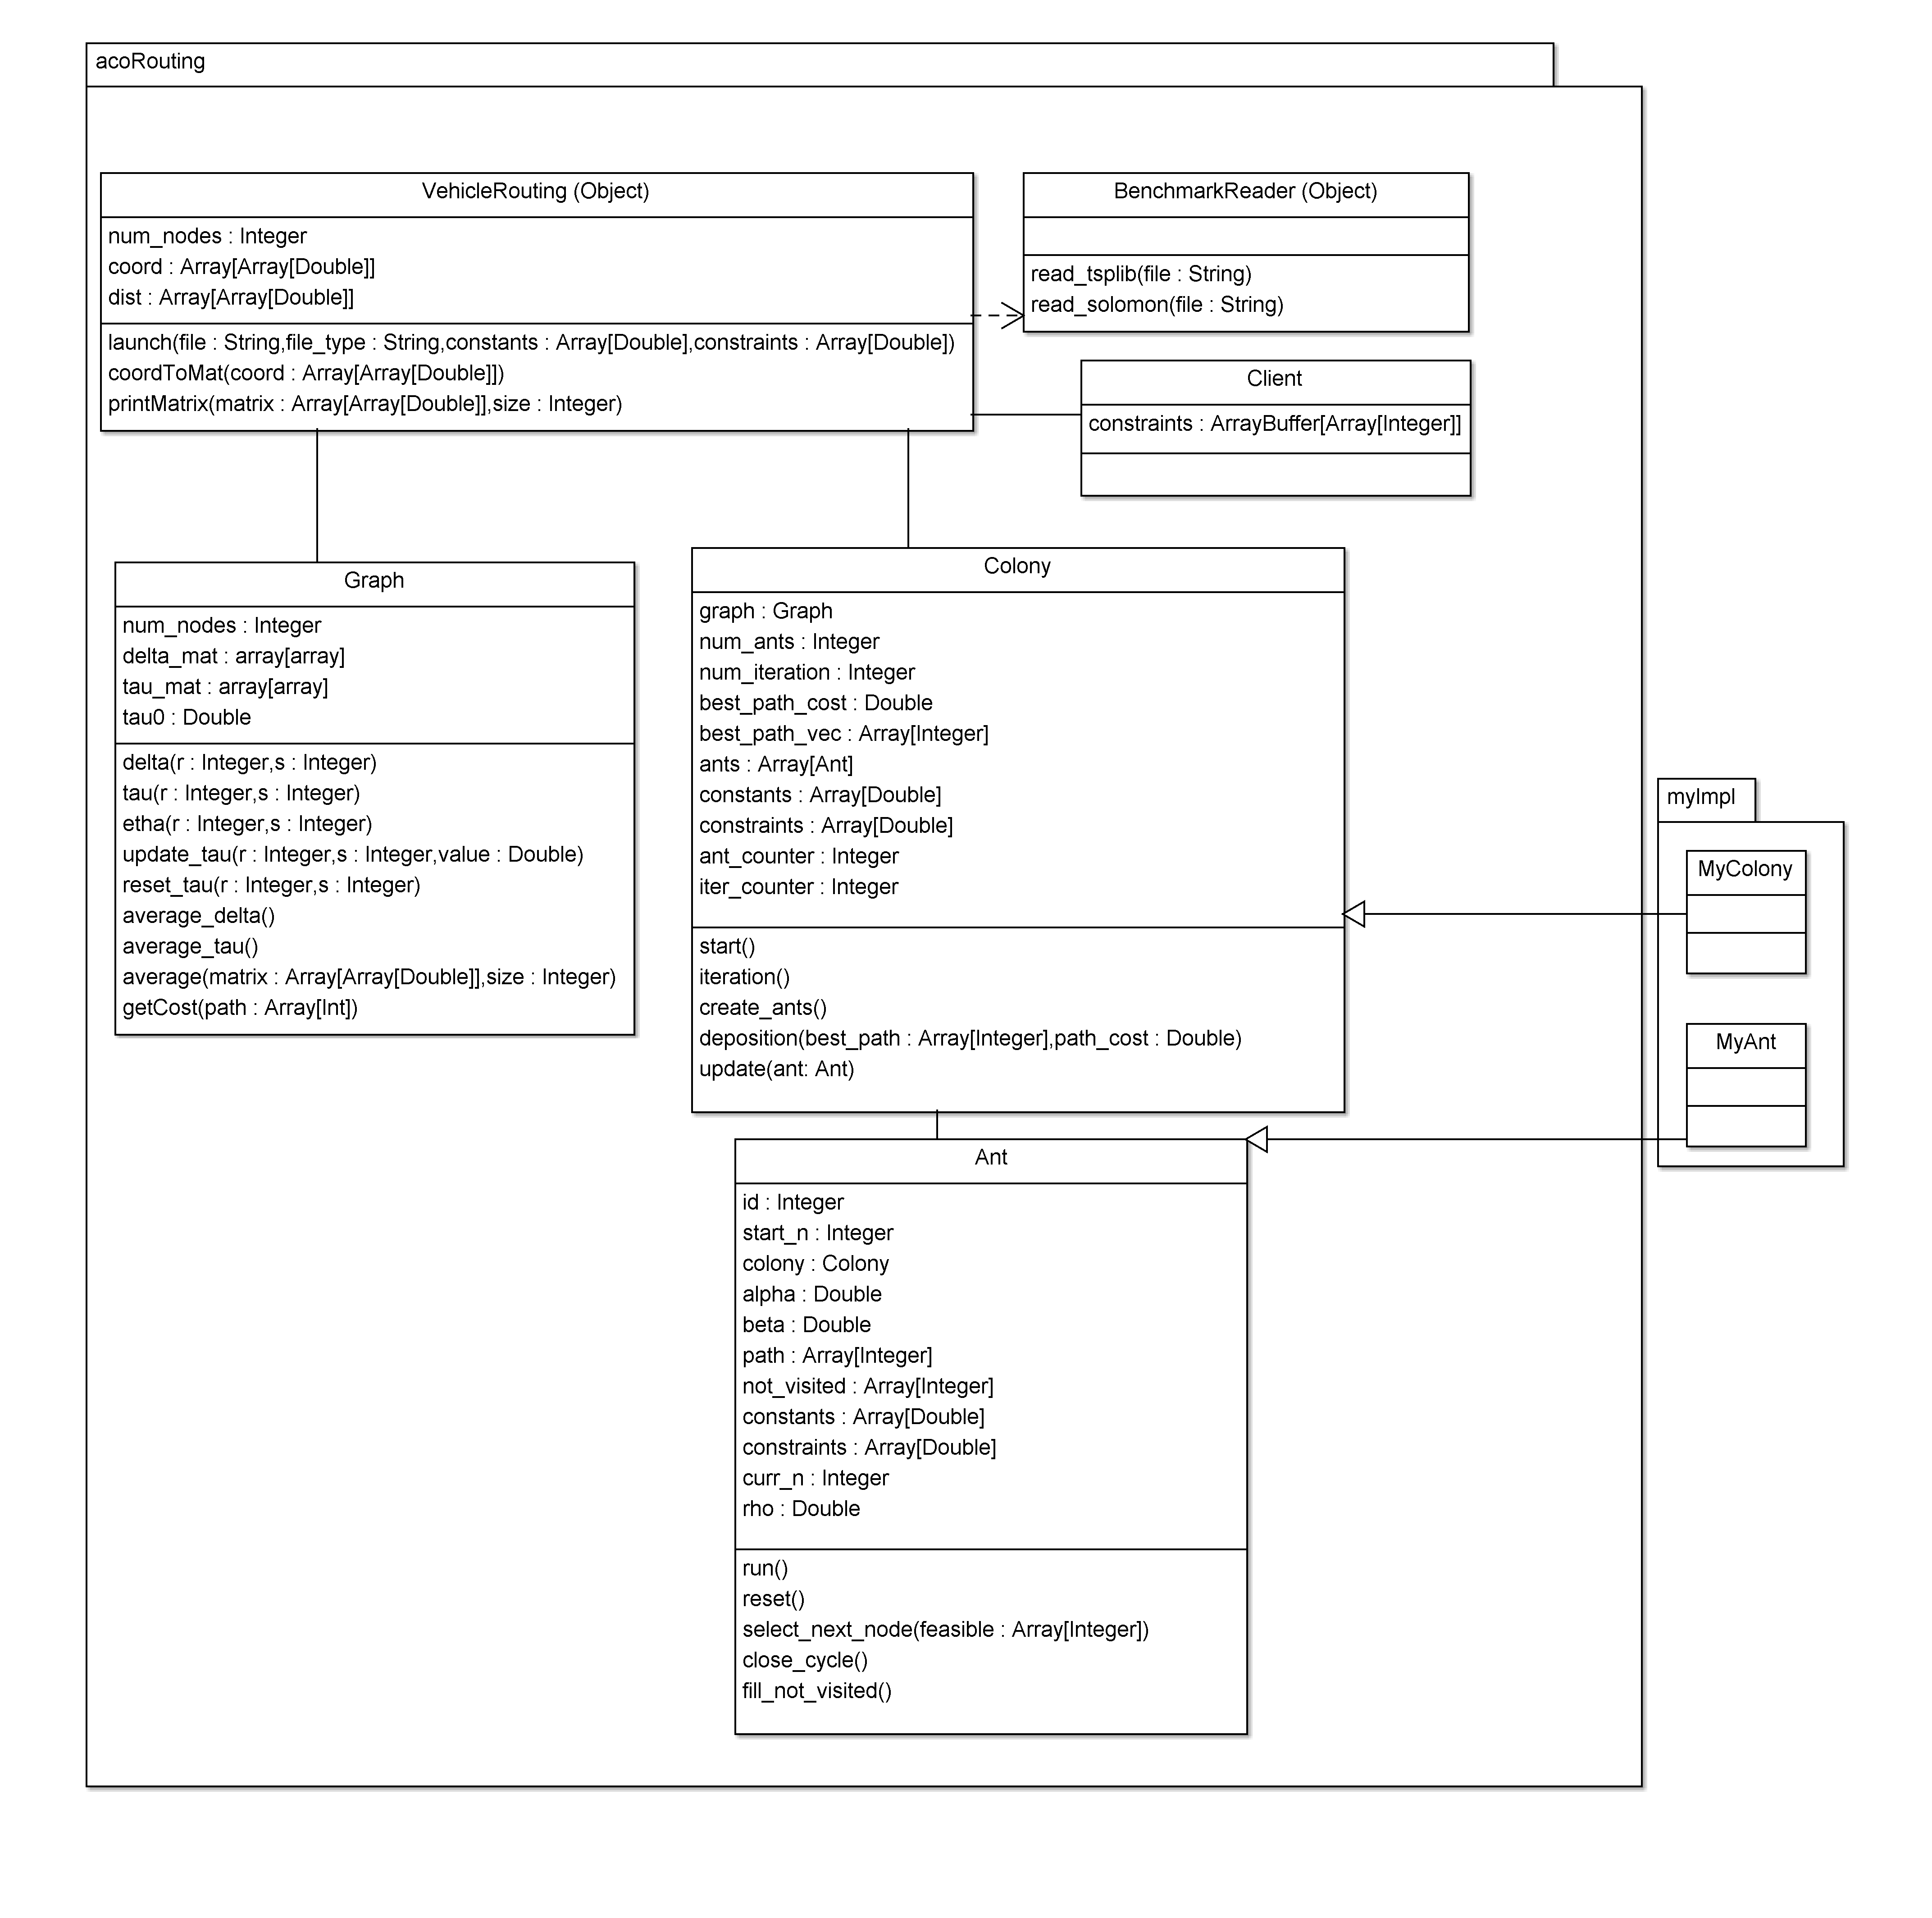
\includegraphics[scale = 0.1]{images/uml.png}
	\caption{UML diagram of the Framework developed.}
	\label{fig:UML}
\end{figure}
%\end{landscape}

\subsection{VehicleRouting object}\label{vrobject}
\begin{figure}
	\centering
		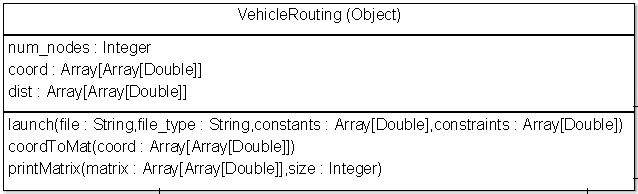
\includegraphics[scale = 0.5]{images/vehiclerouting.png}
	\caption{UML diagram of the VehicleRouting object.}
	\label{fig:vehiclerouting}
\end{figure}
The figure \ref{fig:vehiclerouting} is an UML representation of that object. This object is the "main" object of the framework.  It contains a method \texttt{launch(file:String,...)} that has for purpose of coordinating all the work done by the other classes. It uses the \texttt{FileReader} object methods to read the input file \texttt{file}. Then it transforms the data read into a matrix that will be used to create an instance of the Graph class. Finally it creates an instance of the \texttt{MyColony} class that will be used to find a solution to the problem. The method \texttt{coordToMat()} is used to transform the information contained in the input file that are cartesian coordinates into a distance matrix. A distance matrix is a square matrix $M$ that contains the distance between the city $i$ and $j$ at $M_{ij}$. The parameters of  the launch method are used to fix the number of iterations, the number of ants and other constants that are used in the program.

\subsection{BenchmarkReader object}
\begin{figure}
	\centering
		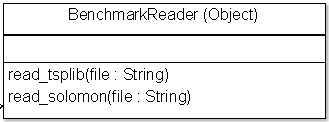
\includegraphics[scale = 0.5]{images/benchmarkreader.png}
	\caption{UML diagram of the BenchmarkReader object.}
	\label{fig:benchmarkreader}
\end{figure}
\texttt{BenchmarkReader} is an object that contains two methods \texttt{read\_tsplib(file)} and \texttt{read\_solomon(file)}. Each method can read a TSPLib file or a SolomonLib file respectively. The way a TSPLib file or SolomonLib file should be encoded is explained in section \ref{howtoframework}. The figure \ref{fig:benchmarkreader} is the representation of that object.

\subsection{Graph class}
\begin{figure}
	\centering
		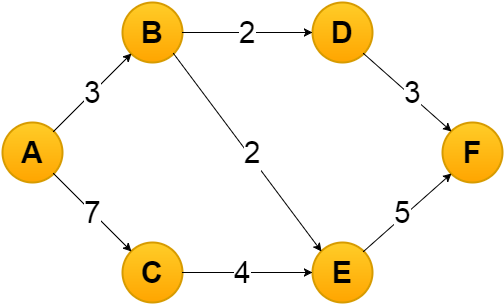
\includegraphics[scale = 0.5]{images/graph.png}
	\caption{UML diagram of the Graph class.}
	\label{fig:graph}
\end{figure}
Graph is a class containing all the information about the graph that represents the problem. This information is stored into the \texttt{delta\_mat} matrix. A Graph object is created by the VehicleRouting object after the input file has been read.
The graph class also contains information about the pheromones because they are held in a similar matrix, \texttt{tau\_mat}. The methods defined in the Graph class are used to access and modify these matrices.

\subsection{Client object}
\begin{figure}
	\centering
		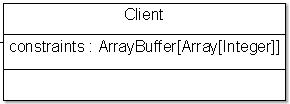
\includegraphics[scale = 0.5]{images/client.png}
	\caption{UML diagram of the Client object.}
	\label{fig:client}
\end{figure}
Client is a data object containing an ArrayBuffer \texttt{constraints} whose goal is to keep all the clients demands and constraints in that single array. The UML representation is in figure \ref{fig:client}.

\subsection{Colony class}
\begin{figure}
	\centering
		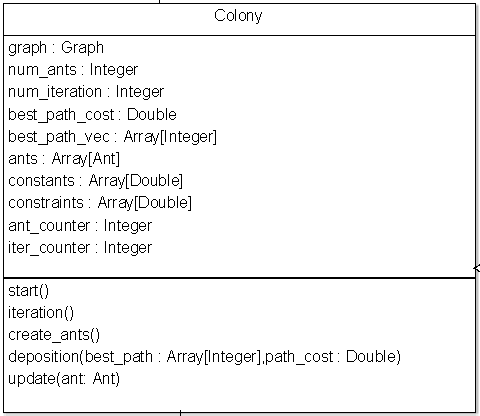
\includegraphics[scale = 0.5]{images/colony.png}
	\caption{UML diagram of the Colony class.}
	\label{fig:colony}
\end{figure}
The class Colony is an important class because it is the class that coordinates all of the ants that are used to solve a problem. The method \texttt{start()} creates all the ants that populate the colony (each ant is an instance of the \texttt{MyAnt class}). Then a loop that runs the ants is done until we reach a maximum fixed number of iterations. In that loop the method \texttt{iteration()} is called. This method runs each ant created using the \texttt{run()} method of these ants. When all ants have built their path, their results are compared and pheromones are dropped using the \texttt{deposition()} method. Finally, the best path is given to the \texttt{VehicleRouting} object that will print it.

\subsection{Ant class}
\begin{figure}
	\centering
	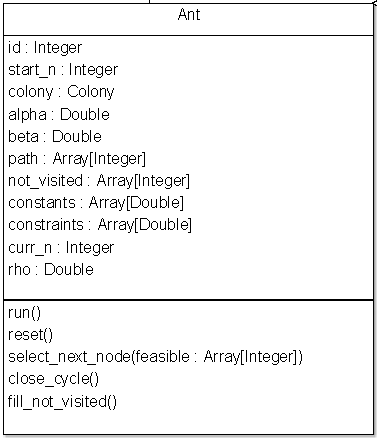
\includegraphics[scale = 0.5]{images/ant.png}
	\caption{UML diagram of the Ant class.}
	\label{fig:ant}
\end{figure}
The Ant class is also an important one because it is the class that controls the behavior of the ant. The core method of this class is the \texttt{run()} method. This method aims to make a path that is a solution to the problem. It will visit the cities one after another until there is no more city to visit. The choice of the next city to visit is made using the \texttt{select\_next\_node()} method. 

\subsection{MyColony - MyAnt}
These classes are intended to the user of the framework. These classes inherit from the \texttt{Colony} and \texttt{Ant} class respectively. The explanations about the way of completing these classes will be given in the next section (section \ref{howtoframework}).

%%%Explication sur les choix d'implémentation tels que le langage utilisé, les représentation des differentes structures de données etc etc.%%
\section{Implementation Choices}
In these sections the choices made for the implementation of the framework are explained. This covers the language used, the representation of the graph, the representation of the clients and the constraints associated to them, the parameters given to the different methods and the base case of the Framework.

\subsection{Language used}
The Scala language was carefully chosen. Scala is high level and a mixed paradigm language, it uses pure object-oriented and functional programming. The fact that it is object oriented allows for the creation of a framework that will be extended by inheritance by the user.

\subsection{Representation of the graph}
In routing problems, we always work with weighted graphs, graphs that have values attached to the edges. These values represent the cost of traveling from one node to the next. When we work with ACO, each ant has to access these values quite frequently. The weighted graph is thus represented as a weighted adjacency matrix. This choice permits to have access to the different value with a $O(1)$ complexity.

Let $v_i$ and $v_j$ be numbered vertices for $1\leq i,j\leq n$. Let $w_{ij}$ be the weight of an edge $e$ and assume that all edge weights are positive ($w_{ij}\geq 0$). Let $M[i,j]$ be an adjacency matrix where $M[i,j] = w_{ij}$ for each edge $e=(v_i,v_j)$. For each vertex $i$ in the graph, $M[i,i]=0$. 

Figure \ref{fig:adjacencymatrix} shows an example of a graph with its matrix representation.

\begin{figure}
	\centering
		\begin{subfigure}[b]{0.3\textwidth}
			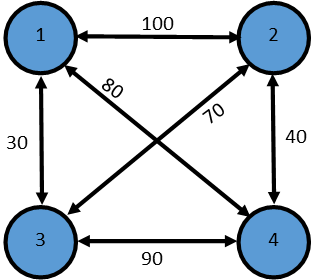
\includegraphics[width=\textwidth]{images/graph1.png}
			\caption{A simple weighted Graph}
		\end{subfigure}
		\qquad
		\begin{subfigure}[b]{0.3\textwidth}
			\begin{tabular}{cccc}
				0 & 100 & 30 & 80\\
				100 & 0 & 70 & 40 \\
				30 & 70 & 0 & 90 \\
				80 & 40 & 90 & 0 \\
			\end{tabular}
			\caption{Weighted adjacency matrix}
		\end{subfigure}
	\caption{A simple graph with its matrix representation}
	\label{fig:adjacencymatrix}
\end{figure}

\subsection{Client constraints}
	To represent the clients and the constraints associated to them, there are two choices: creating a Client class where each client is an instance of that class or creating a single Client object that contains all the information about all the clients of the problem in a single array. Because of the input file that presents the constraints in a sort of array, and because of the fact that an element in an array is accessed in $O(1)$, the second option is chosen.
		
	In the framework, a client Object is used, this object contains an ArrayBuffer named \texttt{constraints}. This ArrayBuffer contains an array for each constraints on the clients. For example, with a VRPTW of size $n$ (i.e.: with $n-1$ clients and 1 depot) the arraybuffer \texttt{constraints} is represented in figure \ref{fig:arraybuffer}. $Q_i$ represents the demand of client $i$. $a_i$ and $b_i$ represent respectively the begining and the end of the time window of the client $i$. If another constraint is added, a new array is added to the ArrayBuffer.
	\begin{figure}%
	\center
	\begin{tabular}{|c|c|c|}
		\hline
		\multicolumn{3}{|c|}{constraints} \\
		\hline
		0 & 1 & 2 \\
		\hline
		$Q_0$ & $a_0$ & $b_0$ \\
		$Q_1$ & $a_1$ & $b_1$ \\
		... & ... & ...\\
		$Q_n$ & $a_n$ & $b_n$ \\
		\hline
	\end{tabular}
	\caption{An example of the constraints arraybuffer}%
	\label{fig:arraybuffer}%
	\end{figure}
	
\subsection{Parameters of the launch method}\label{param}
	As explained in section \ref{vrobject}, the launch method has different parameters. The first is the location of the input file \texttt{file}. Then a string \texttt{file\_type} that says wich type of file is given in parameter (i.e.: Solomon or TSPLIB). The third and fourth are two arrays named \texttt{constants} and \texttt{constraints}. These arrays, as their names indicates, will contain the values of the constants used by the programs and the values associated to the constraints.
	
	The choice of an array to keep these values is made because it is flexible. If the user of the framework needs to use constants, he just has to pass an array that defines these constants. The same goes for the constraints. These two arrays are passed to the Colony and Ant instances. This also permits to the user to make a program that takes these arrays as parameters, so it is easy to manipulate and modify these constants.
	
	The \texttt{constants} array has a fixed minimum size. Some values, such as the number of ants to be used and the maximum number of iterations, must be the first two in the array. See figure \ref{tab:constants} for an example of the \texttt{constants} array.
	
	\begin{table}%
	\centering
	\begin{tabular}{|c|c|c|c|c|}
	\hline
	\# Ants & \# Iterations & $\alpha$ & $\beta$ & ...\\
	\hline
	\end{tabular}
	\caption{Representation of the \texttt{constants} array.}
	\label{tab:constants}
	\end{table}
	
	The \texttt{constraints} array is an array that is used by the ants to fix the limits that are given on the constraints. For example, in a CVRP, the ants (i.e. the trucks) have a maximum capacity limit. This limit is given in the constraints tabular. If other constraints of the same type must be added, this array is extended.
	
\subsection{Colony and Ant class}
	The ants that build solutions share common information, the pheromone matrix. This matrix is modified by the ants when they use an arc, and also when they all have completed a tour. This is where the colony class is important. The colony class collects the information about all the tours that the ants built, compares them and updates the pheromones using the best solution built by the ants.
	These two classes are also the base classes that will be extended by an user of the framework. The question is what contains these classes? 
	To answer that, we can make a first observation : The CVRP and the VRPTW are two generalizations of the TSP. Indeed, a TSP is a CVRP that has one vehicle with no capacity limit and customer with no demand. The same goes for the VRPTW, a TSP is a VRPTW with one vehicle, no capacity limit, no time limit and customer with no demand and infinite time-windows. 
	This observation leads to the implementation of the base problem (the TSP) in the base classes. This permits a user to directly use the framework without coding anything on a TSP problem. 
	In these classes can be found the methods that apply the base algorithm of an ACO system. These methods should not (or rarely) be modified. This is the \texttt{start()} and \texttt{iteration()} methods of the colony that are presented in the code block \ref{code:start} and the \texttt{run()} method of the ant presented in the code block \ref{code:run}. 
	
	\subsubsection{Colony}
	
	\begin{lstlisting}[captionpos=b, caption = Source code of the start and iteration method in Colony class, label= code:start]
def start() {
  this.create_ants
  while (!this.done) {
    this.iteration()
  } 
}

def iteration() {
  this.ant_counter = 0
  this.iter_counter += 1
  for (i <- 0 to num_ants - 1) {
    ants(i).run
  }
  this.deposition(this.best_path_vec, this.best_path_cost)
  if (this.best_path_cost < VehicleRouting.best_cost){
    VehicleRouting.best_tour = this.best_path_vec
    VehicleRouting.best_cost = this.best_path_cost
  }
  this.best_path_vec = Array(0)
  this.best_path_cost = Double.MaxValue
}
\end{lstlisting}
This fraction of code is a scala implementation of the ACO algorithm given in algorithm \ref{alg:acometa}. The Colony starts by creating the artificial ants. Then each ant is launched and does its work. When all the ants have made their tour, the best tour is used to drop pheromone with the \texttt{this.deposition()} method. If the best path found during this iteration is better than the best path found at the moment, it is replaced.


\subsubsection{Ant}
	
\begin{lstlisting}[captionpos=b, caption = Source code of the run method in Ant class, label= code:run]	
def run() {
  var new_node = 0
  while (this.not_visited.length != 0) {
    new_node = this.select_next_node(this.not_visited, null)
    this.path_cost += graph.delta(this.curr_n, new_node)
    this.path = this.path :+ new_node
    (this.graph.update_tau(curr_n, new_node, (1 - this.rho) 
		   * this.graph.tau(curr_n, new_node) 
			   + (this.rho * this.graph.tau0)))
    this.curr_n = new_node
  }
  close_cycle()


  this.colony.update(this)
  this.reset
}
\end{lstlisting}

The fraction of code presented in code block \ref{code:run} is the core method of the Ant. The \texttt{run()} method goal is to build a path that is a solution to the problem. The method iterates while the \texttt{not\_visited()} array is not empty. At each iteration:
\begin{itemize}
	\item a new node is selected
	\item the node is added to the path
	\item a local pheromone update is done according to equation \ref{eq:localpheromone}.
	\item the current node is replaced by the new selected node.
\end{itemize} 
When the iteration is done, the cycle is closed (the salesman goes back to his start point) and the results are sent to the Colony.


\section{How to use the framework}\label{howtoframework}
Now that we have a clear idea of the design of the framework, we will discover the convention governing its proper use. To do that, the correct way to use the framework to solve a CVRP problem will be elaborated. Some aspects change from the TSP base implementation of the framework. A capacity constraint is added. The Input file, the Client class and obviously the Colony and Ant classes change. The modifications are explained hereafter. 

\subsection{Input File}
The input file describing the problem must follow the convention of the TSPLIB file or the convention of the Solomon benchmark.
\subsubsection{TSPLIB}
The TSPLIB input file contains two part : a \emph{specification part} containing information on the file format and its content, and a \emph{data part} containing explicit data as the distances between cities. \cite{tsplib}
\paragraph{The specification part} contains :
\begin{itemize}
	\item the \emph{name} of the file.
	\item the \emph{type} of problem it describes (TSP, CVRP,...).
	\item the \emph{dimension} of the problem (Total number of nodes and depot in the case of a CVRP).
	\item the \emph{capacity} that specifies the truck capacity in a CVRP.
	\item the other constraints that can be added and their limitation on a truck.
	\item the \emph{edge weight type} that specifies how the distances are given.
\end{itemize}
\paragraph{The Data part} contains : 
\begin{itemize}
	\item the \emph{node\_coord\_section} where node coordinates are given in the form:
	\begin{verbatim}
	<integer> <real> <real>
	\end{verbatim}
	\item the \emph{depot\_section} that contains the list of depot nodes (always node 0 in our case)
	\item the \emph{demand\_section} that contains the demands of all nodes of a CVRP. It is given in the form: 
	\begin{verbatim}
	<integer><integer>
	\end{verbatim}
	\item the other constraints per node.
\end{itemize}

\subsubsection{Solomon Benchmark file}
The Solomon benchmark takes the form of a matrix. Each row contains all the information about a node. Table \ref{tab:Solomon} demonstrates the contents of the rows of that matrix.

\begin{table}%
\centering
\tiny
\begin{tabular}{l|l|l|l|l|l|l|l}
Client\_Number & X\_coordinate & Y\_coordinate & Demand & Ready\_Time & Due\_Date & Service\_Time & ... \\
\end{tabular}
\caption{A row of a Solomon benchmark file}
\label{tab:Solomon}
\end{table}
More columns can be added if there are more constraints to represent.
\cite{solomon}

\subsection{Constraints}
The CVRP is a TSP augmented with capacity constraints on the vehicle and demand of the client. In this section, we discover how to adapt the framework to solve the CVRP problem.
 
\subsubsection{Modelization of the constraints}
As outlined above, the CVRP adds one constraint to the TSP. It is the constraint bound to the capacity of the vehicle. 
The first change to make is of course in the input file. As explained before, a new set of data is added for each client: the demand.
The next changes we have to do are in the implementation of the Colony and the Ant. To do that, the class \texttt{MyAnt} and \texttt{MyColony} that \textbf{extends} the \texttt{Ant} and \texttt{Colony} class have to be implemented. 
\paragraph{The MyColony} class does not need many new methods. As the Ants do not start from a random city like in the TSP, but rather from the depot, the method \texttt{create\_ants()} is modified. The code of the \texttt{MyColony} class is presented in code block : \ref{code:colonycvrp}.

\begin{lstlisting}[captionpos=b, caption = MyColony implementation for a CVRP, label= code:colonycvrp]
class MyColony(graphp: Graph, num_antsp: Int, num_iterationp: Int) 
       extends Colony(graphp, num_antsp, num_iterationp) {

  override def create_ants() {
    var startcity = 0
    this.ants = Array.empty[MyAnt]
    for (i <- 0 to (num_ants - 1)) {
        startcity = 0
    var ant = new MyAnt(i, startcity, this, VehicleRouting.capacity)
        ants = ants :+ ant
    }
    ants
  }
}
\end{lstlisting}
\paragraph{The MyAnt} class needs more modifications. The capacity constraint has to be taken into account when selecting the next node. To do that, different methods are possible. The simplest is to follow the selection process as for the TSP and send the truck back to the depot if the selected node violates the constraints. In that case, only the \texttt{select\_next\_node()} method must be overridden. Below is the new implementation of the \texttt{select\_next\_node()} method.
\begin{lstlisting}[captionpos=b, caption = MyAnt implementation for a CVRP, label= code:antcvrp]
override def select_next_node(feasable: Array[Int]): Int = {
    val graph = this.graph
    var new_node = -1
    var denominator = 0.0

    if (feasable(0) == 0) { 
      return 0
    }
    if (!feasable.isEmpty) {
      denominator = compute_denominator(feasable)
      new_node = choose_new_node(denominator, feasable)
      if (new_node == -1) {
        new_node = this.curr_n
      }
      if (this.capacity < Client.constraints(0)(new_node) + this.load) {
        new_node = 0
        this.load = 0
      } else {
        this.load += Client.constraints(0)(new_node)
        this.not_visited = this.not_visited.filterNot(_ == new_node)
      }
      return new_node
    } else {
      new_node = 0
      this.load = 0
      return new_node
    }
  }
\end{lstlisting}

\subsection{Adding new Constraints}
In this section, through two other examples, it is shown how to add other constraints to a CVRP. The two examples that are described in this section will be tested in chapter \ref{tests}. 

The first example concerns the adding of a constraint to a CVRP that is verified after a tour is built. In other words, an ant constructs a valid path according to the capacity constraint. This path must then be validated to be sure it does not violate other constraints. This type of constraint is used in some vehicle routing problems with black box feasibility (3D loading ...) \cite{massen2013vrp}. This type of constraint is called "off-parcour constraint".

The second example concerns the adding of a soft constraint that is used in the construction of a tour. We talk about a soft constraint because the constraint will be used in the evaluation of the quality of a solution provided (i.e. in the objective function). A soft constraint can not be violated but must be taken into account in the building of a solution to have a correct solution. This type of constraint is called "in-parcour constraint".

The third example is a hard "in-parcour constraint". What is called a hard constraint is, as the capacity of a CVRP, a constraint that can not be violated.

\subsubsection{Off-parcour constraint}
	In this section is explained the adding of an off-parcour constraint. In this example, a simple rule is implemented but the case can be generalized to any more complex rules. In this example, the rule forbids two cities that have consecutive numbers to be visited one after the other. In other words, a city $i$ can not be visited after city $i-1$ or city $i+1$.
	
	To implement this rule, from the CVRP implementation given above, we only need to modify the \texttt{MyColony}. Indeed, the \texttt{MyAnt} class does not need modifications because the constraint that we add can not be verified in the path construction but only when the path is finished. 
	
	When an ant has finished building a path, the colony has to test whether or not the path is the shortest found in this iteration and whether or not the path is valid according to the rule we defined. This is done with both methods \texttt{update(ant:Ant)} and \texttt{is\_valid(ant:Ant)}. The code of these functions is given in code block \ref{code:offconstraint}.
	
	\begin{lstlisting}[captionpos=b, caption = Method used for the off-path constraints, label= code:offconstraint]
 override def update(ant:Ant){
    this.ant_counter += 1
    if(is_valid(ant)){
      if (ant.path_cost < this.best_path_cost) {
        this.best_path_cost = ant.path_cost
        this.best_path_vec = ant.path
      }
    }
  }  
  def is_valid(ant:Ant):Boolean={
    var last=0
    for(c <- ant.path ){
      if (last != 0){
        if(last+1 == c || last-1 == c){
          return false
        }
      }
      last=c
    }
    return true
  }\end{lstlisting}

The method \texttt{update(ant:Ant)} is called every time an ant has build a path. The update method checks first if the path is valid using the \texttt{is\_valid(ant:Ant)} then keeps the solution of the ant if it is the best of the iteration. If the path is not valid, it is discarded. In this case the method \texttt{is\_valid(ant:Ant)} is quite simple but it can be replaced by something different easily.

\subsubsection{In-parcour constraint}\label{inconstraints}
\paragraph{The soft constraint} that is implemented is a preference for the client to be placed first in a subtour. Each client has a value assigned to him that represents how important it is to be the first in a subtour. The value of that preference is an integer in the range $0$ through $10$, $10$ symbolizing a great need to be first and $0$ symbolizing the fact that a client does not want to be first.

To implement that constraint, the first thing to do is to add the preference of each client in the input file. Once this is done, the \texttt{MyAnt} class must be modified to take the constraint into account. A different random proportional rule will be used when the ant is at the depot (that is the city $i = 0$). Instead of using the classical one presented in equation \ref{eq:cvrp proportional rule}, when at city $i = 0$ a new factor is added to the equation to take into account the preferences of each client. The new rule that is used is :
\begin{equation}
	p_{0j}^k =
	\begin{cases}
		\frac{[\tau_{0j}]^\alpha [\eta_{0j}]^\beta [\xi_{j}]^\epsilon}{\sum_{l\in N_i^k}{[\tau_{0l}]^\alpha [\eta_{0l}]^\beta [\xi_{l}]^\epsilon}} & \text{if } j\in N_i^k\\
		0 & \text{otherwise}
	\end{cases}
\label{eq:modifproportionalrule}
\end{equation}
where $\xi_{j}$ is the value associated with client $j$ and $\epsilon$ is a constant as $\alpha$ and $\beta$ that affects the importance of $\xi$ in the building of a solution. As $\epsilon$ is a constant, the value of that constant is added into the array \texttt{constants} presented in section \ref{param}.

The second thing to change is the objective function that measures the quality of a tour in the \texttt{MyColony} class. To do that, instead of taking only the length of the path to give a cost to a solution, we add to that cost a value related to the preference of each first client in a subtour (see code block \ref{code:soft}).

\begin{lstlisting}[captionpos=b, caption = Taking the preference into account , label= code:soft]
  override def update(ant: Ant) {
    this.ant_counter += 1
    var first_in_tour = new ArrayBuffer[Int]
    var cost = ant.path_cost
    for (i <- 0 to ant.path.length-1){
      if(ant.path(i)==0){
        first_in_tour += ant.path(i+1)
      }
    }
    for (a<-first_in_tour){
      cost += ((math.abs(Client.constraints(1)(a)-10))*100)
    }
    if (cost < this.best_path_cost) {
      this.best_path_cost = cost
      this.best_path_vec = ant.path
    }
  }
	\end{lstlisting}
	
	Again this example is a simple one. The objective function and the proportional rule used are maybe not the best in that case, but the goal of this example is just to show how to add constraints and what it implies in the implementation.

\paragraph{The hard constraint} that is implemented here is a limit on a sub-path of a CVRP solution. As a reminder, a CVRP solution is a set of paths where each path begins and ends at the depot and visits some cities. To the classic CVRP that limits only the capacity of a vehicle, we add here a limit on the maximum length of a subpath. This limit can represent, for example, the size of the fuel tank of a truck. Adding that kind of constraint is done by modifying the ant behaviour. This is done in the implementation of the \texttt{MyAnt} class by overriding the \texttt{select\_next\_node(feasable:Array[Int])} method. In the implementation of the CVRP given above, we force the ant to go back to the depot if the next node selected in the path violate the constraint capacity. To take the new constraint into account, we simply need to calculate and keep in memory the length of the subtour, and send the truck back to the depot if the constraint is violated (if the subtour is too long).
In this example the \texttt{constraints} array that is defined as an argument in the \texttt{launch} method of the VehicleRouting object (see section \ref{param}) will contain a new value that will represent the maximum length of a tour.



\chapter{Experimental Results}\label{tests}
%!TEX root = ../main.tex
This chapter presents the tests made on the framework and their results. First, the TSP is tested, which is the base case of the framework. Next, a classical CVRP implementation and a VRPTW implementation are tested. After that, an example of CVRP with new constraints relative to the client is tested, and finally, an example with path constraint is tested.
These tests have two goals, the first is to compare the efficiency of the ACO implementation, the second is to test the framework by giving tests examples on extended CVRP (CVRP with new constraints). To achieve that, the tests are run with a configuration that is a good compromise between the computation time and the solution quality. The configuration is the value  that is given to different constants like the number of ants, iterations ,$\alpha$, $\beta$ ... The values given have been found in the literature and by testing.

All the tests are made on a personal computer with Intel Core i7-3610 CPU that runs at 2.30 GHz.

\section{The Traveling Salesman Problem}
These first series of tests permit to determine the efficiency of the base implementation of the framework. The tests are made with problems of different sizes that we can find in TSPLIB \cite{tsplib}. Four different tests of different size are made. 
The TSP problems that are used are :
\begin{description}
\item[eil51] A TSP with 51 cities by Christofides
\item[berlin52] A TSP that represents 52 locations in Berlin.
\item[eil76] A TSP with 76 cities by Christofides 
\end{description}

These instances of TSP are chosen over the others from the TSPLIB because they have been tested with other ACO implementations and thus we can compare similar results together. Each instance of the TSP problem is tested a hundred times.
In table \ref{tab:mytsp}, the results of the tests are listed. In table \ref{tab:acstsp}, the results obtained by two other implementations \cite{dorigo1997acs} \cite{hlaing2011ant} are presented. In the implementation \cite{dorigo1997acs} 1250 iterations and a number $N$ of ants that is equal to the number of cities in the problem are used. No similar information has been found for the implementation \cite{hlaing2011ant}.

As a reminder, here is the signification of the names of the columns:
\begin{description}
\item[\#iterations] denotes the number of iterations made.
\item[\#ants] denotes the number of ants used.
\item[$\alpha$] is a parameter influencing the use of the pheromone
\item[$\beta$] is a parameter influencing the importance of the heuristic function.
\item[mean] is the mean value of the path length of the 100 trials.
\item[best] is the best value of the path length of the 100 trials.
\end{description}

\begin{table}%
\centering
\small
\begin{tabular}{|l|l|l|l|l|l|l|}
\hline
problem & \#iterations & \#ants & $\alpha$ & $\beta$ & mean & best \\
\hline
\hline
eil51 & 500 & 51  & 5.0 & 5.0 & 451.48 & 430.34  \\
\hline
berlin52 & 500 & 52  & 5.0 & 5.0& 7730.00 & 7544.36\\
\hline
eil76 & 500 & 76 & 5.0 & 5.0 & 592.27 & 567.96  \\
\hline
\end{tabular}
\caption{results of the tests for the four TSP instances}
\label{tab:mytsp}
\end{table}



\begin{table}%
\centering
\begin{tabular}{|l|l|l|}
\hline
Implementation & problem & best \\
\hline
ACS \cite{dorigo1997acs} & eil51 & 427.96\\
& eil76 & 542.37 \\
ACO for TSP \cite{hlaing2011ant} & eil51 & -- (426) \\
& berlin52 & 7544.36 (7542)\\
& eil76 & -- (538) \\ 
\hline
\end{tabular}
\caption{results of other ACO implementation for the TSP}
\label{tab:acstsp}
\end{table}

The values that are in brackets are rounded values. They are calculated with rounded distances.

The results of the TSP implementation are quite good. Compared with the ACS algorithm developed by M.Dorigo and L.M.Gambardella, the results are almost the same. The same goes for the implementation of Hlaing and Khine.

Tests are not made on TSP instances with more cities because, in order to have good results, new functions have to be made to improve the results. For example, a local search method or a structure known as candidate list must be implemented. A candidate list is a preselection of nodes that can be elected at each step by an ant. With the framework, if these functions are encoded, it can be easily added by modifying the class \texttt{MyAnt}.

\section{The Capacitated Vehicle Routing Problem}\label{testcvrp}
As for the TSP, the instances of CVRP that are tested are choosen so that they can be compared to other ACO implementations. The instances that are used come from the problem described by Christofides, Mingozzi and Toth. In particular their problem: 
\begin{description}
	\item [C1] A CVRP with 51 cities and a truck capacity of 160.
	\item [C3] A CVRP with 101 cities and a truck capacity of 200.
	\item [C4] A CVRP with 151 cities and a truck capacity of 200.
\end{description}
The results of the framework are compared with the results of J.Bell and P.McMullen \cite{bell2004ant} and Y.Bin, Y.Zhong-Zhen and Y.Baozhen \cite{yu2009improved}. These two tests are run with a number of 5000 iterations and a fixed number of 30 ants. In table \ref{tab:mycvrp} are listed the results obtained with the ACO framework and in table \ref{tab:acocvrp} the results of the scientists given above.

\begin{table}[h]
\centering
\small
\begin{tabular}{|l|l|l|l|l|l|l|}
\hline
problem & \#iteration & \#ants & $\alpha$ & $\beta$ & mean & best \\
\hline
\hline
C1 & 500 & 51 & 5.0 & 5.0 & 587.23 & 556.75  \\
\hline
C3 & 500 & 100 & 5.0 & 5.0 & 983.26 & 942.38  \\
\hline
C4 & 500 & 100 & 5.0 & 5.0 & 1272.34 & 1269.65 \\
\hline

\end{tabular}
\caption{results of the tests for the CVRP}
\label{tab:mycvrp}
\end{table}

\begin{table}[h]
\centering
\begin{tabular}{|l|l|l|l|}
\hline
implementation & problem & mean & best \\
\hline
\hline
\cite{bell2004ant} & C1 & 528.90 & 524.80 \\
& C3 & 865.65 & 854.20 \\
& C4 & 1143.43 & 1131.83\\
\hline
\cite{yu2009improved} & C1 & 524.61 & 524.61\\
& C3 & 844.32 & 830.00 \\
& C4 & 1042.52 & 1028.42\\
\hline
%\cite{tan2012ant} & C1 &  \\ %% pourcentages a transformer. a faire..
%\hline
\end{tabular}
\caption{results of other ACO implementation of CVRP}
\label{tab:acocvrp}
\end{table}
The solutions provided by the framework are within $10\%$ of the optimum of other ACO algorithms. This can be explained by several factors. First, the number of iterations used is much greater in the implementations \cite{bell2004ant} \cite{yu2009improved} where they set the number of iterations to $5000$ than here in the tests where we set the number of iterations to $500$. Next, these implementations have special local search algorithms and use candidate lists to improve the results, the framework implementation tested here does not (but again, if the functions are encoded, the framework can easily be extended). Finally, the test with 151 cities is already quite large for a basic implementation thus it is normal to observe bad results.


\section{Vehicle Routing Problem with Time Windows}
The VRPTW benchmark tested are instances of the Solomon benchmark \cite{solomon}. The implementation made in the framework is a simplified version of the MACS-VRPTW \cite{gambardella1999macs}. The results obtained are compared to the original MACS-VRPTW version. In the simplified version, we omit the local search function and an insertion function that are implemented in the MACS-VRPTW. The results obtained with the framework are presented in table \ref{tab:myvrptw}, the ones obtained with the MACS implementation are presented in table \ref{tab:macsvrptw}. Values in brackets represent the number of vehicles used. The number of iterations used by \cite{gambardella1999macs}  is fixed with a computational time limit. As it is implemented in C++ and uses multi-threading at its maximum, the comparaison is hard to make.

\begin{table}[h!]
\centering
\small
\begin{tabular}{|l|l|l|l|l|l|l|l|}
\hline
problem & \#iterations & \#ants & $\alpha$ & $\beta$ & mean  & best \\
\hline
\hline
R101.25 & 500 & 25 & 5.0 & 5.0 & 889.51 (10) & 802.95 (10)  \\
\hline
R101.50 & 500 & 50 & 5.0 & 5.0 & 1567.08 (18) & 1446.07 (18)  \\
\hline
\end{tabular}
\caption{results of the tests for the VRPTW}
\label{tab:myvrptw}
\end{table}

\begin{table}[h!]
\centering
\begin{tabular}{|l|l|l|}
\hline
implementation & problem & best  \\
\hline
\hline
MACS-VRPTW & R101.25 & 617.1 (8) \\
& R101.50 & 1044.0 (12) \\
\hline
\end{tabular}
\caption{results of the MACS implementation of VRPTW}
\label{tab:macsvrptw}
\end{table}

As can be seen, the simplified implementation of the framework has bad results. This can be explained by the fact that the insertion function plays an important role in the construction of solutions that minimize the number of vehicles used. That function was not clearly described in the paper of Gambardella, but again, if we have that function, it can be easily added to the framework and thus improve the results.

\section{CVRP with in-path constraints}
This section will present two CVRP problems with new constraints added in the construction of a solution. These constraints are called "in-path" constraints because they have an effect on the construction of the solution by the ant. This type of constraint is opposed to the "off-path" type where a path is validated or not based on the finished path. 

The first test simulates a constraint on the truck. The trucks used for the vehicle problem have a limited fuel capacity. Thus a sub-path can not have a length greater than a certain value $tour\_length$. The adding of that constraint is done as explained in section \ref{howtoframework}. 

The second test simulates a preference of the clients who want to be first in a tour. Each client is assigned a value $pref$ from $1$ to $10$. Clients with high value are clients that need to be first in a tour and clients with low values are clients that do not want to be first in the tour. Both tests are performed on the C1 instance of the CVRP presented in section \ref{testcvrp}. The results of these tests are listed in the table \ref{tab:vrpin}. 


\paragraph{Limited subpath} For the test, the maximum subpath is set to 50. In the best case there are eleven vehicles. The best result of the problem C1 given in section \ref{testcvrp} had 10 vehicles and a total length of 556. Here with a limitation of the subtours of 50, with a simple calculation, it points out that at least 11 vehicles are needed. The length of the complete path is almost doubled. This can be explained by the fact that when new vehicle are used, there are more trips between the depot and the cities. An analysis of the different paths given by the 100 executions of the problem reveals that all the constraints are always verified as expected.

\paragraph{Client preference} The constraint has been implemented in a soft way. The goal here is to satisfy the most clients but it is not always possible. The objective function that gives a score to a solution has thus been modified (see section \ref{inconstraints}). The score takes into account the total distance (as in the usual CVRP) and the respect of the preference. The best path and the preference associated with client of interest are given in table \ref{tab:path} (as a reminder 0 represent the depot).  As can be seen in that table, the first clients of each tour have high preferences. The other nodes and preferences of each subtour are not reported as the preference is only taken into account for the first client visited after a depot.
\begin{table}
\centering
\small
\begin{tabular}{|l|l|l|l|l|l|l|l|}
\hline
problem & \#iterations & \#ants & $\alpha$ & $\beta$ & mean & best  \\
\hline
\hline
limited sub-path & 500 & 50 & 5.0 & 5.0 & 919.66 & 881.37 (18) \\
\hline
First client pref. & 500 & 50 & 5.0 & 5.0 & 710.14 & 614.00  \\
\hline
\end{tabular}
\caption{results of the CVRP implementation with in-path constraints}
\label{tab:vrpin}
\end{table}

\begin{table}
\centering
\begin{tabular}{|l|l|}
\hline
best path & preference \\
\hline
\hline
 0 & \\
 46 & 6\\
 47 & \\
 ... &\\
 0 & \\
 48& 7\\
 8& \\
 ...&\\
 0 & \\
 17 &10 \\
 37& \\
 ...&\\
 0 & \\
 4 & 10 \\
 44& \\
 ...&\\
\hline
\end{tabular}
\caption{results of the CVRP implementation with in-path constraints}
\label{tab:path}
\end{table}

This test shows that it is possible to add a constraint on the path in an easy way. It also shows that the constraint tends to be respected. The path is different from the classic CVRP presented earlier, and the constraint added modifies the path. In table \ref{tab:path}, we can see that the first cities of a tour have a high preference as expected.

\section{CVRP with off-parcour constraints}
The "off-parcour" constraints are constraints that can only be verified after the construction of a tour. As for example in a VRP with 3D-loading constraints where some rules must be verified to validate a path. Here a simple rule is implemented but this simple rule can be replaced by a more complex one. The rule forbids two cities having consecutive numbers to be visited one after the other. In other words, a city $i$ can not be visited after city $i-1$ or city $i+1$. A simple function verifies a path and indicates if it is valid or if it must be discarded. The result of that implementation on the C1 CVRP instance is given in table \ref{tab:cvrpoff}. An analysis on the path given after the execution of the test proves that the constraint is verified. The best result is different of the normal C1 instance because, in the best solution of that problem, there are several consecutive nodes.

Interestingly, the problem has been modified with a new constraint and so the result slightly differs from the original instance of the CVRP. It shows again that the constraint added have an effect on the results produced and are respected.

\begin{table}
\centering
\small
\begin{tabular}{|l|l|l|l|l|l|l|l|}
\hline
problem & \#iterations & \#ants & $Q_0$ & $\alpha$ & $\beta$ & mean & best  \\
\hline
\hline
off-parcour & 500 & 50 & 0.9 & 5.0 & 5.0 & 634.09 & 601.55  \\
\hline
\end{tabular}
\caption{results of the CVRP implementation with off-path constraints}
\label{tab:cvrpoff}
\end{table}

\chapter{Conclusion}
%!TEX root = ../main.tex



%% <== End of core
%%%%%%%%%%%%%%%%%%%%%%%%%%%%%%%%%%%%%%%%%%%%%%%%%%%%%%%%%%%%%



%%%%%%%%%%%%%%%%%%%%%%%%%%%%%%%%%%%%%%%%%%%%%%%%%%%%%%%%%%%%%
%% BIBLIOGRAPHY AND OTHER LISTS
%%%%%%%%%%%%%%%%%%%%%%%%%%%%%%%%%%%%%%%%%%%%%%%%%%%%%%%%%%%%%
%% A small distance to the other stuff in the table of contents (toc)
\addtocontents{toc}{\protect\vspace*{\baselineskip}}

%% The Bibliography
%% ==> You need a file 'bibliographie.bib' for this.
%% ==> You need to run BibTeX for this (Project | Properties... | Uses BibTeX)
\addcontentsline{toc}{chapter}{Bibliography} %'Bibliography' into toc
\nocite{*} %Even non-cited BibTeX-Entries will be shown.
\bibliographystyle{ieeetr} %Style of Bibliography: plain / apalike / amsalpha / ...
\bibliography{bibliography} %You need a file 'literature.bib' for this.

%% The List of Figures
\clearpage
%%\addcontentsline{toc}{chapter}{List of Figures} %%no need in the toc
\listoffigures

%% The List of Tables
\clearpage
%%\addcontentsline{toc}{chapter}{List of Tables} %% no need in the toc.
\listoftables


%%%%%%%%%%%%%%%%%%%%%%%%%%%%%%%%%%%%%%%%%%%%%%%%%%%%%%%%%%%%%
%% APPENDICES
%%%%%%%%%%%%%%%%%%%%%%%%%%%%%%%%%%%%%%%%%%%%%%%%%%%%%%%%%%%%%
\appendix
%% ==> Write your text here or include other files.

%\input{FileName} %You need a file 'FileName.tex' for this.
%%!TEX root = ../main.tex
\begin{verbatim}
NAME : A-n32-k5
COMMENT : (Augerat et al, No of trucks: 5, Optimal value: 784)
TYPE : CVRP
DIMENSION : 32
EDGE_WEIGHT_TYPE : EUC_2D 
CAPACITY : 100
NODE_COORD_SECTION 
 1 82 76
 2 96 44
 3 50 5
 4 49 8
 5 13 7
 6 29 89
 7 58 30
 8 84 39
 9 14 24
 10 2 39
 11 3 82
 12 5 10
 13 98 52
 14 84 25
 15 61 59
 16 1 65
 17 88 51
 18 91 2
 19 19 32
 20 93 3
 21 50 93
 22 98 14
 23 5 42
 24 42 9
 25 61 62
 26 9 97
 27 80 55
 28 57 69
 29 23 15
 30 20 70
 31 85 60
 32 98 5
DEMAND_SECTION 
1 0 
2 19 
3 21 
4 6 
5 19 
6 7 
7 12 
8 16 
9 6 
10 16 
11 8 
12 14 
13 21 
14 16 
15 3 
16 22 
17 18 
18 19 
19 1 
20 24 
21 8 
22 12 
23 4 
24 8 
25 24 
26 24 
27 2 
28 20 
29 15 
30 2 
31 14 
32 9 
DEPOT_SECTION 
 1  
 -1  
EOF 
\end{verbatim}

\end{document}

